\documentclass[../../main.tex]{subfiles}

\begin{document}
    
    \section{Steganalysis}
    Steganalysis is the branch os study dedicated at analysing the methods and the vectors used to transmit an hidden message in order to retrieve such message whenever it is present.
    Unlike chryptanalysis where the message may even be apparent but enchrypted, in steganalysis the study of the message starts from a suspect.
    \subsection{Methods}
    Hereinafter we will present the two type of methods used in steganalysis in order to obtain the secret message 

    \subsubsection{Statistical}

    \subsubsection{Structural}
    

    \subsection{Images}


    \subsection{Audio}
    
    
    \subsection{Text}
    
    
    \subsection{TCP/IP}
    \subsubsection{Introduction}
    Before treating such topic we must briefly discuss the behaviour of the TCP/IP (\textbf{Internet protocol suit}) communications.
    
    \textbf{IP (Internet Protocol)} is at the basis of internet communication. The protocol exploits the principle of encapsulation, sending packets composed by a \emph{header} which contains information such as the \textbf{destination address} and \textbf{source address} and a \emph{payload}
    which represents the actual data to be transmitted. Since physical channels usually have a limited \emph{MTU}\footnote{Maximum Transmission Unit}, then the data is usually fragmented in smaller chunks, wrapped into an header and only then transmitted.
    
    \textbf{TCP (Transmission Control protocol)} is a protocol used for reliable(little information loss), ordered, error-checked data transmission between a machine
    hosting the data (\textbf{Server}) and another requiring such data (\textbf{Client}). It is performed previous a three-way handshake which estabilishes a connection between server and client, thus preparing 
    a reliable communication channel.

    \textbf{UDP (User Datagram Protocol)}, contrary to TCP, is less reliable but faster.
     It broadcasts the data in an unordered and uncontrolled way to the receiver. 
    There is no need to estabilishing a connection in order to implement such protocol.

    \begin{figure}[h]
        \centering
        \caption{Structure of TCP packet}
        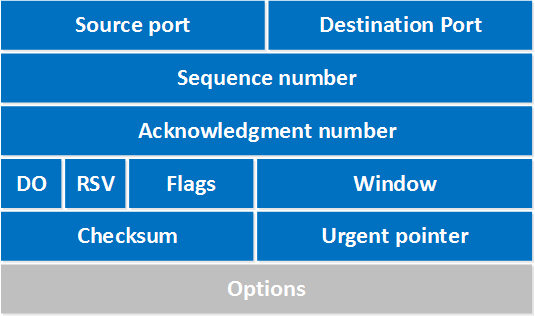
\includegraphics[scale=0.5]{tcp_header.png}
    \end{figure}

    \begin{figure}[h]
        \centering
        \caption{Structure of TCP packet}
        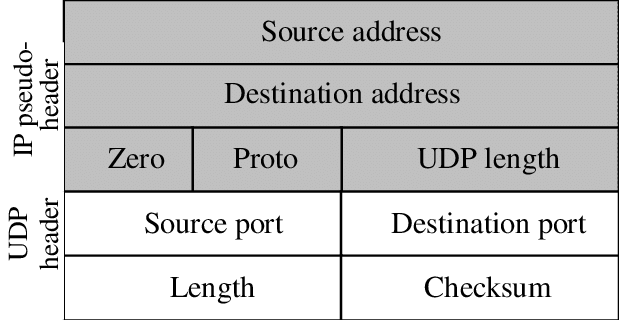
\includegraphics[scale=0.]{udp_header.png}
    \end{figure}

    \pagebreak

    \subsubsection{Exploits and protection tools}

    As you could notice from the previous figures, the first part of the header is the same. This is because it is part of the IP protocol itself.
    In the second part of each header we find different types of metadata which are specific for each protocol. Generally the metadat contained in the header is redundant 
    for the transmission of the message itself and this redundancy may become a target for a \emph{stego-algorithm}\footnote{an algorithm used for steganography} which starting from a 
    \emph{cover-network packet sequence}\footnote{a sequence of packets which will be transmitted over the network acting as a cover for the hidden messace} and a \emph{covert message}, can generate a sequence of packets(each one embedding a portion of the covered message) which will be sent over the network.

    This procedure is not a \emph{risk-free} approach for the attacker who wishes to send the \emph{cover-network packet sequence}, since it is possible that the data will be currupted during transmission or there could be losses using non-reliable transport protocols(UDP).
    Other criticalities of such method stay in the fact that the sequence of packets will most likely traverse multiple nodes in the network before reaching the target, and the message may be detected by these nodes.

    The defense against Steganography in TCP/IP communication consists in a series of standards which are implemented by the devices on the internet and that we will illustrate through some examples.


    \textbf{Tof(Type of service)} bits are a field in the TCP header which are nowdays rarely used. This could open doors to a steganographic attack if modern operating systems did not set them to zero by default. A warden monitoring the channel could immediately signal an error.

    \textbf{IP ID} is a field in the Internet Protocol which is used to assist the receiver in reassemblying the fragmented packets. This field consist of randomly unique numbers representing a packet.
    It is possible to insert other types of information in this field by simply conform to the uniqueness constraint. Since in many cases the numbers used for the IP ID are not random, by knowing the charachteristics of the sender it is possible
    to detect an infiltration.

    \textbf{IP Fragment Offset} is an offset which is present in the IP header which helps the receiver to reconstruct the sequence of bits from the fragmented sequence.
    Modulating the size of the fragments changes the offset field in the header and thus a message could be sent. The protection against this method is simply checking the size of the packets relative to the MTU and so even
    in this case a warden can easily detect an error.

    \textbf{TCP sequence number} is a field in the TCP header which stores the randomly chosen position(for security reasons) of the first byte to be transmitted through the channel. The steganographic method consists in replacing this field with the data to be sent.
    Being random it is more difficult to spot a breach in the channel. In this case the usage of a \emph{SVM}\footnote{Support Vector Machine}, a machine learning tool able to identify patterns inside the data transmitted could come into hand.
    However an error could be detected even simply by checking the presence of repetitions in the stream(not admitted by design). 

    \textbf{Timestamp modulation} is another technique of steganography which operate by modifing the \emph{LSB}\footnote{Least Significant bit} of the timestamp of a TCP packet in order to represent a '1'.
    The covert message is thus embedded into the data stream. Since the TCP Timestamp support is not universal, machines not supporting such feature may detect the hidden message.

    \pagebreak
\end{document}